\documentclass[28pt]{article}

\usepackage[margin=1in]{geometry}
\usepackage[utf8]{inputenc}
\usepackage[spanish]{babel}
\usepackage{fontspec}%Cambiar fuente
\usepackage{color}
\usepackage{amsmath}
\usepackage[dvipsnames]{xcolor}%Lista de nombres de colores: http://www.maths.adelaide.edu.au/anthony.roberts/LaTeX/ltxusecol.php

\usepackage{tcolorbox}%Ecuaciones en recuadro
\tcbuselibrary{theorems}%Ecuaciones en recuadro

\usepackage{lipsum}%Texto de prueba
%-----Linea horizontal de color----------------------
\newlength{\seplinewidth}
\newlength{\seplinesep}
\setlength{\seplinewidth}{1mm}
\setlength{\seplinesep}{2mm}
\colorlet{sepline}{Salmon}
\newcommand*{\sepline}{%
  \par
  \vspace{\dimexpr\seplinesep+.5\parskip}%
  \cleaders\vbox{%
    \begingroup % because of color
      \color{sepline}%
      \hrule width\linewidth height\seplinewidth
    \endgroup
  }\vskip\seplinewidth
  \vspace{\dimexpr\seplinesep-.5\parskip}%
}
%-------------------------------------------------------------------
\setmainfont{Letters for Learners}[
              SizeFeatures={Size=13},
              % ... other options ...
            ]

%Use: {\fontspec{FUENTE NAME}Texto con otra fuente} para tener textos
%con otra fuente distinta a la establecida en \setmainfont
%--------------------------------------------------------------------

\title{\textbf{{\fontspec{Dulcelin}Electromagnetismo II\\Tarea 3}}}
\author{\textbf{{\fontspec{Dulcelin}Jessica Martínez Marcelo}}}
\date{Marzo, 2020}

\begin{document}
\maketitle

\sepline
    {\color{RedViolet}
      1. Se tiene un trozo de material dieléctrico, como se muestra en la Figura \ref{fig:fig1}. En su interior hay 3 conductores con cargas $Q_{1}$, $Q_{2}$ y $Q_{3}$ respectivamente y superficies correspondientes $S_{1}$, $S_{2}$ y $S_{3}$.\\Considere la superficie gaussiana $S$ de la figura y aplique la Ley de Gauss para la carga total que encierra, que es: $Q_{T}=Q_{1}+Q_{2}+Q_{3}+Q_{p}$, donde $Q_{p}$ es la carga de polarización del dieléctrico, tanto volumétrica como superficial.\\Utilice el teorema de la Divergencia y demuestre con detalle que:
      \begin{equation}
        \oint_S \left(\epsilon_{0}\bar{E}+\bar{P}\right) \cdot d\bar{a}=Q_{libre}
      \end{equation}
      Donde $Q_{libre}=Q_{1}+Q_{2}+Q_{3}$ es la carga libre total depositada en los conductores y $\bar{P}$ es la polarización del dieléctrico punto a punto $\bar{P}=\bar{P}(\bar{r})$.
      \\
      A la ecuación (1) se le conoce como la Ley de Gauss para dieléctricos. Usualmente se define un vector $\bar{D}=\epsilon_{0}\bar{E}+\bar{P}$, y:
      \begin{equation}
        \oint_S \bar{D}(\bar{r}) \cdot d\bar{a}=Q_{libre}
      \end{equation}
    }

\begin{figure}[h!]
  \centering
    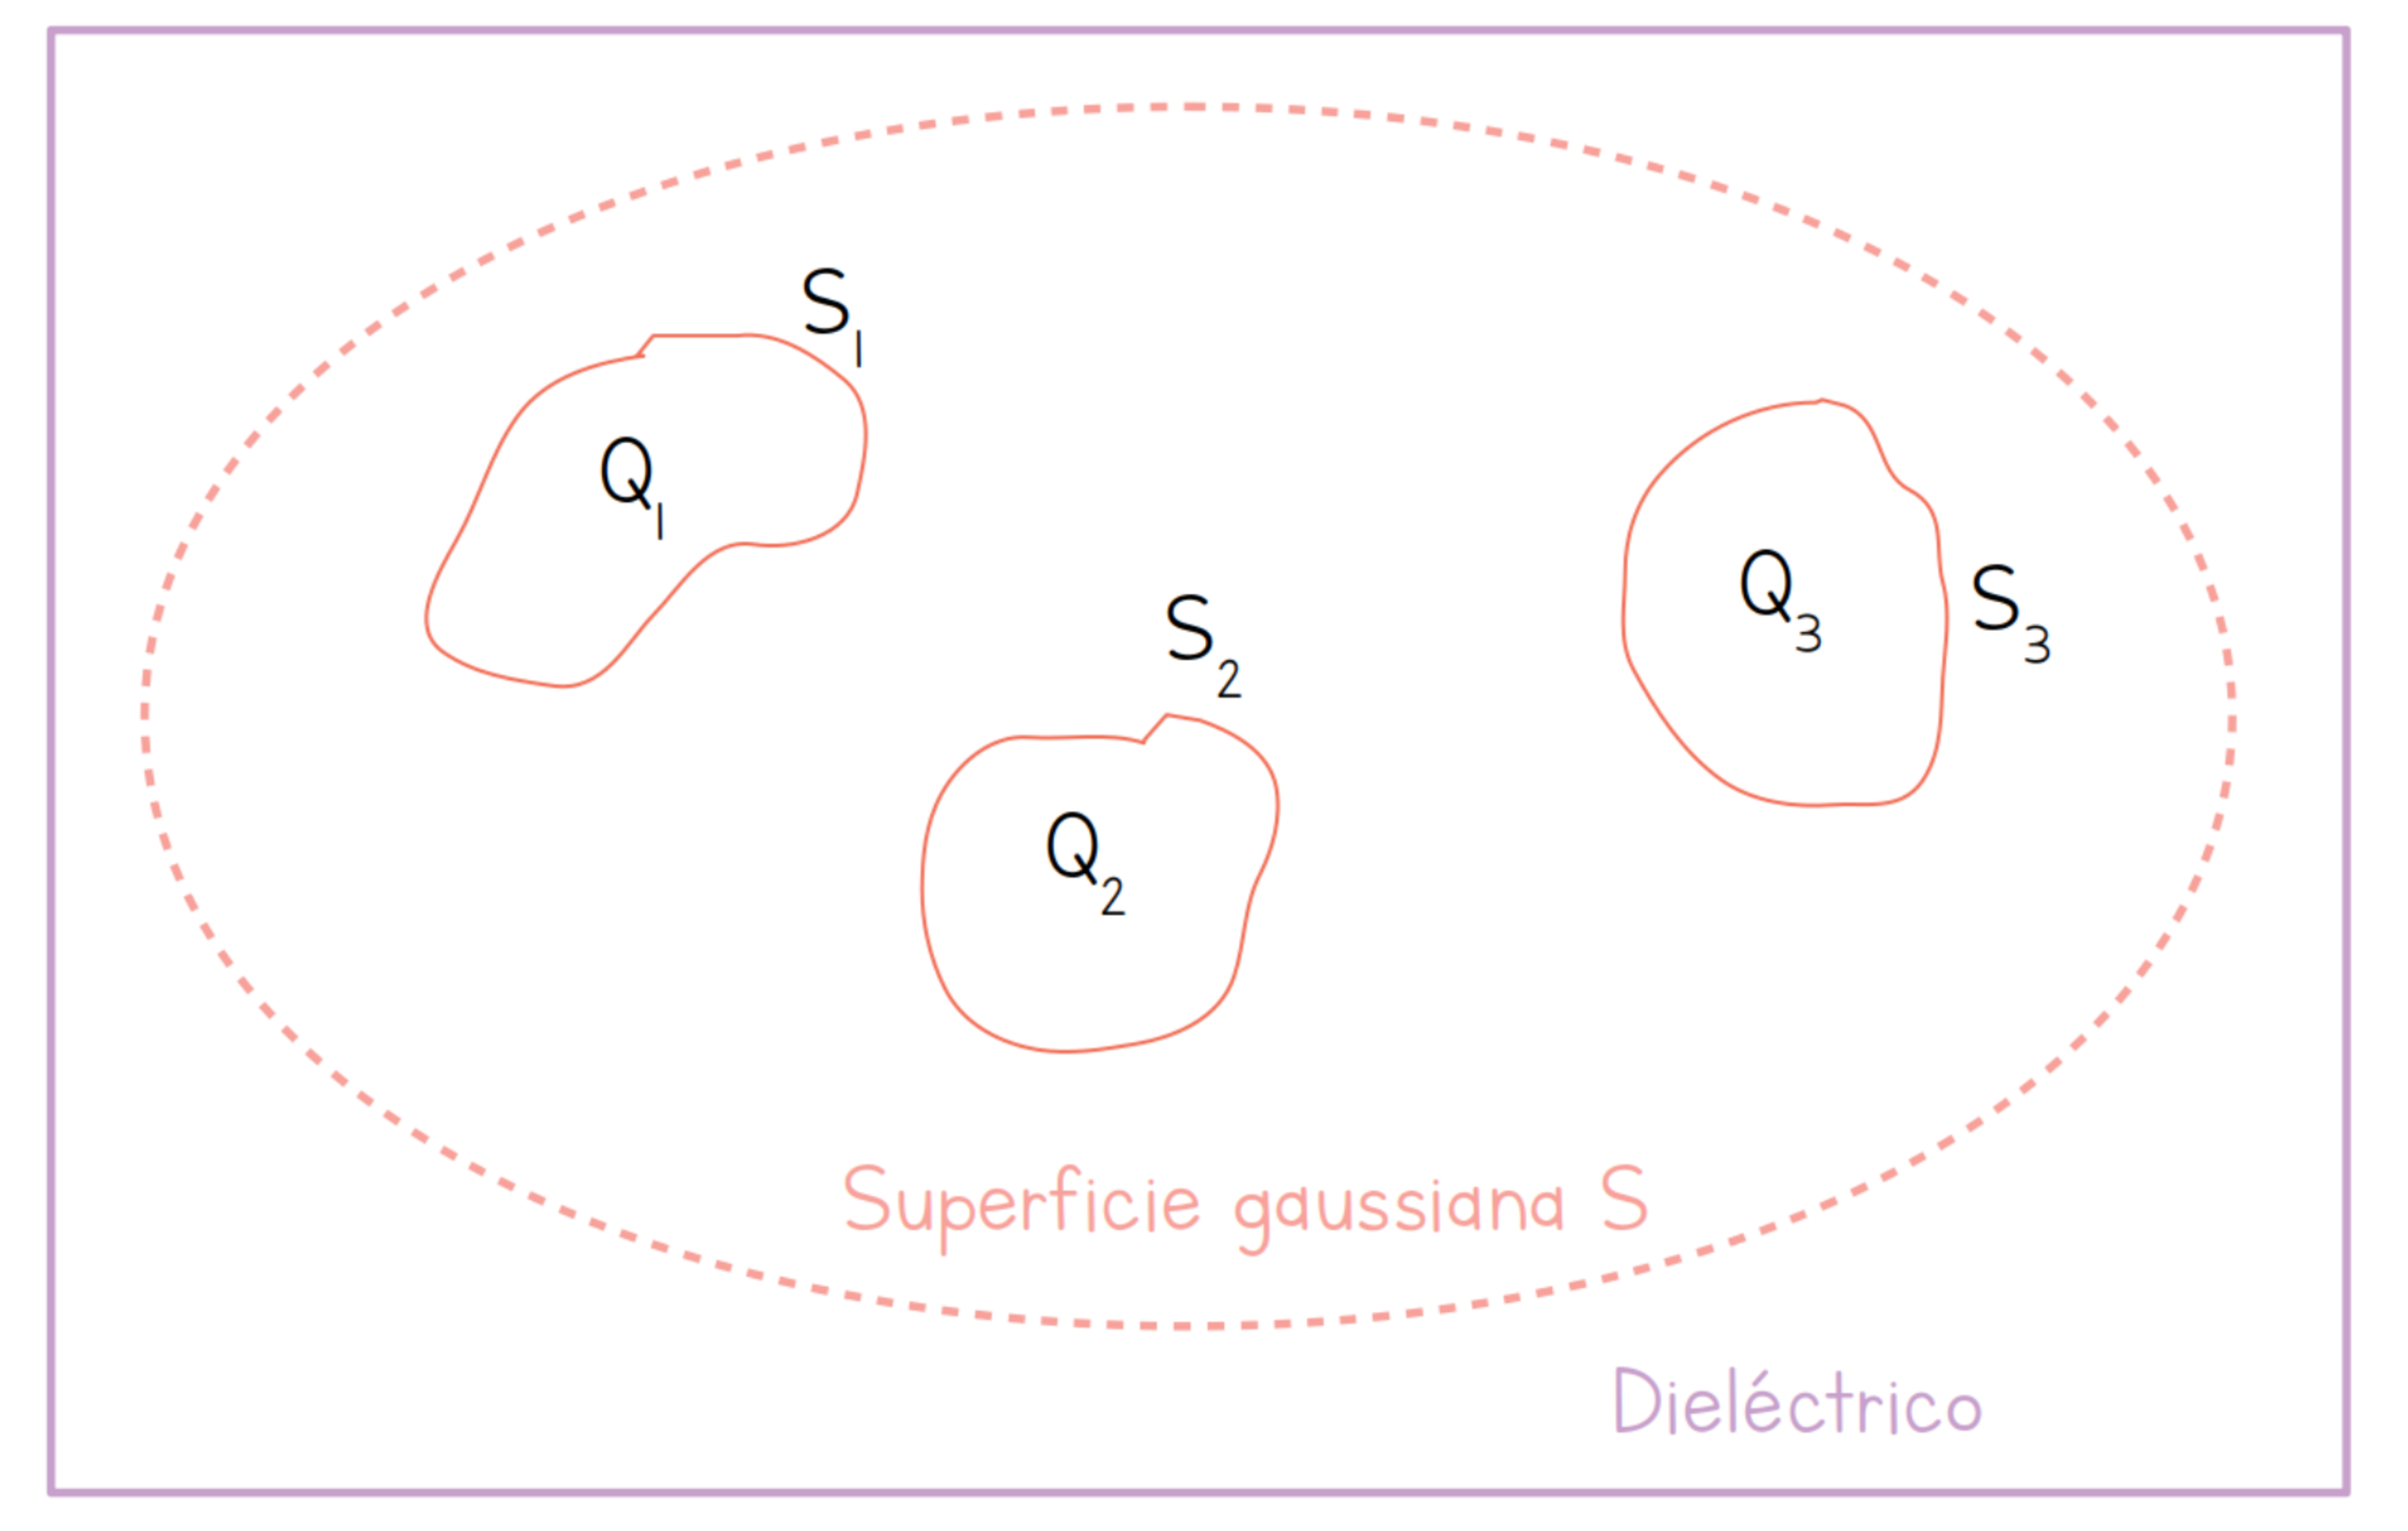
\includegraphics[width=6cm]{figures/fig1}
  \caption{Dieléctrico.}
  \label{fig:fig1}
\end{figure}

{\color{WildStrawberry}Solución:}
\\
Aplicando la Ley de Gauss se tiene:
\begin{equation}
  \oint_S \bar{E} \cdot \bar{n}\,da=\frac{1}{\epsilon_{0}}\left( Q_{libre}+Q_{p}\right)
\end{equation}
además la carga de polarización neta $Q_{p}$ está dada por:
\begin{equation}
  Q_{p}=\int_{S_{1}+S_{2}+S_{3}}\bar{P} \cdot \bar{n}\,da + \int_{V}(-\bar{\nabla}\cdot \bar{P})\,dv
\end{equation}
Con $V$ el volumen del del dieléctrico encerrado por $S$. Dado que no hay una frontera del material dieléctrico en $S$, la integral de superficie en la ecuación (4) no contiene una contribución de $S$. \\
Usando el teorema de la Divergencia en el segundo sumando de (4), y cuidando incluir las contribuciones de todas las superficies que limitan a $V$, es decir $S$, $S_{1}$, $S_{2}$ y $S_{3}$, se tiene:
\begin{equation}
  Q_{p}=\int_{S_{1}+S_{2}+S_{3}}\bar{P} \cdot \bar{n}\,da-\oint_S \bar{P}\cdot \bar{n}\,da-\int_{S_{1}} \bar{P}\cdot \bar{n}\,da-\int_{S_{2}} \bar{P}\cdot \bar{n}\,da-\int_{S_{3}} \bar{P}\cdot \bar{n}\,da
\end{equation}
entonces:
\begin{equation}
  Q_{p}=-\oint_S \bar{P}\cdot \bar{n}\,da
\end{equation}
Así, sustituyendo (6) en (3) se tiene:
\begin{equation}
  \oint_S \bar{E} \cdot \bar{n}da=\frac{1}{\epsilon_{0}}\left( Q_{libre}-\oint_S \bar{P}\cdot \bar{n}\,da\right)
  \end{equation}
de manera que:
\begin{equation}
  \oint_S \left( \epsilon_{0}\bar{E}+\bar{P} \right) \cdot \bar{n}\,da=Q_{libre}
\end{equation}

Definiendo el vector de {\color{WildStrawberry}desplazamiento eléctrico}: $\bar{D}=\epsilon_{0}\bar{E}+\bar{P}$, como sugiere el problema, se llega finalmente a:
\begin{equation}
  \tcboxmath[colback=Salmon!25!white,colframe=Salmon, title=\centering Ley de Gauss en un dieléctrico:]
	{ \oint_S \bar{D}(\bar{r}) \cdot d\bar{a}=Q_{libre}}
\end{equation}
\sepline%Horizontal line
{\color{RedViolet}
  2. Demuestre (por medio del Teorema de la Divergencia) que en un dieléctrico sin cargas libres en su interior ni en su superficie: $Q_{p}\equiv$carga de polarización:
  \begin{equation}
    %\begin{align}
      Q_{p}=0
    %\end{align}
    \end{equation}
  Con:
  \begin{equation}
    Q_{p}=\int_{S\,\,frontera\,\,de\,\,V}\sigma_{p}\,da+\int_{V}\rho_{p}\,dV
  \end{equation}
  \begin{align}
    \sigma_{p}& =\bar{P} \cdot \hat{n}      &   \rho_{p}&=-\bar{\nabla}\cdot \bar{P}
  \end{align}
}
\\
\\
{\color{WildStrawberry}Solución:}
\\
Sustituyendo las ecuaciones de (12) en (11) se tiene:
\begin{equation}
  Q_{p}=\int_{S\,frontera\,de\,V}(\bar{P} \cdot \hat{n})\,da+\int_{V}(-\bar{\nabla}\cdot \bar{P})\,dV
\end{equation}
Aplicando el teorema de la divergencia en el segundo sumando de (13) se obtiene:
\begin{equation}
  Q_{p}=\int_{S\,frontera\,de\,V}(\bar{P} \cdot \hat{n})\,da-\int_{S\,frontera\,de\,V}(\bar{P} \cdot \hat{n})\,da
\end{equation}
por lo que, en un dieléctrico sin cargas libres en su interior ni en su superficie:
\begin{equation}
  \tcboxmath[colback=Salmon!25!white,colframe=Salmon]%, title=\centering Ley de Gauss en un dieléctrico:]
	{Q_{p}=0}
\end{equation}
\\

\sepline
{\color{RedViolet}
  3. Considerando a un dieléctrico cuya polarización responde linealmenteal campo eléctrico aplicado:$\bar{P}(\bar{r})=\chi \bar{E}(\bar{r})$, donde $\bar{E}(\bar{r})$ es el campo en el dieléctrico, $\chi$ es una constante. Demuestre que:
\begin{equation}
  \bar{D}(\bar{r})=\epsilon \bar{E}(\bar{r})
\end{equation}
con $\epsilon=k \epsilon_{0}$ y $k$ es la constante dieléctrica definida por: $k=1+\frac{\chi}{\epsilon_{0}}$ y que $\bar{P}(\bar{r})=\epsilon_{0}(k-1)\bar{E}$
}
\\
\\
  {\color{WildStrawberry}Solución:}
\\
El vector de desplazamiento eléctrico $D$ se había definido ya en el problema 1. como:
\begin{equation}
  \bar{D}(\bar{r})=\epsilon_{0}\bar{E}(\bar{r})+\bar{P}(\bar{r})
\end{equation}
Si la polarización del dieléctrico respone linealmente entonces:
\begin{equation}
  \bar{D}(\bar{r})=\epsilon_{0}\bar{E}(\bar{r})+\chi \bar{E}(\bar{r})
\end{equation}
Dadas las definiciones de las variables en el problema:
\begin{equation*}
  \epsilon=k \epsilon_{0}\,\,\,y\,\,\,k=1+\frac{\chi}{\epsilon_{0}}\,\, \rightarrow \,\, \epsilon=\left( 1+\frac{\chi}{\epsilon_{0}}\right)\,\, \rightarrow \,\, \epsilon=\epsilon_{0}+\chi \,\, \rightarrow \,\, \epsilon_{0}=\epsilon-\chi
\end{equation*}
sustituyendo la última igualdad en (18):
\begin{equation}
  \bar{D}(\bar{r})=(\epsilon-\chi)\bar{E}(\bar{r})+\chi \bar{E}(\bar{r})=\epsilon \bar{E}(\bar{r})-\chi \bar{E}(\bar{r})+\chi \bar{E}(\bar{r})
\end{equation}
por lo tanto:
\begin{equation}
  \tcboxmath[colback=Salmon!25!white,colframe=Salmon, title=\centering D en medios isótropos:]
	{\bar{D}(\bar{r})=\epsilon \bar{E}(\bar{r})}
\end{equation}
\sepline
{\color{RedViolet}
  4. Considere una carga puntual $Q$ en un fluido dieléctrico de constante $k$. Demuestre que:
  \begin{equation}
    \bar{E}(\bar{r})=\frac{Q}{4\pi k \epsilon_{0}r^{2}}\hat{\mu}_{r}\,\,\,\,\,y\,\,\,\,\,\bar{P}(\bar{r})=\frac{(k-1)Q}{4\pi k\,r^{2}}\hat{\mu}_{r}
  \end{equation}    
}
\\
\\
  {\color{WildStrawberry}Solución:}
\\
De las ecuaciones desarrolladas en los problemas anteriores se sabe que los vectores $\bar{E}$, $\bar{D}$ y $\bar{P}$ son paralelos entre sí en cada punto, además el campo no cambia su forma radial, por lo que sigue existiendo la misma simetría que se tiene en el caso de una carga en el vacío, de esta manera, se puede aplicar la ley de Gauss a una esfera de radio $r$ con la carga $Q$ en el centro:
\begin{equation*}
  \oint_S \bar{D} \cdot \hat{n}\,da=Q \,\,\, \stackrel{\hat{n}=\hat{r}}{\hbox to 25pt{\rightarrowfill}} \,\,\,\oint_S \bar{D} \cdot \hat{r}\,da=Q \,\,\, \stackrel{\bar{D} \parallel \hat{r}}{\hbox to 25pt{\rightarrowfill}} \,\,\,\oint_S D\,da=Q \,\,\, \stackrel{\rm simetría}{\hbox to 40pt{\rightarrowfill}} \,\,\,\ D \oint_S da=Q 
\end{equation*}
Dado que la superficie es una esfera de radio $r$:
\begin{equation*}
  D(4\pi r^{2})=Q\,\,\, \rightarrow \,\,\, D=\frac{Q}{4 \pi r^{2}}
\end{equation*}
Se sabe que la dirección del campo $\bar{D}$ es radial, entonces:
\begin{equation}
  \bar{D}=\frac{Q}{4 \pi r^{3}}\bar{r}
\end{equation}
De esta manera, usando la ecuación (20) y que $\epsilon=k \epsilon_{0}$ se tiene:
\begin{equation*}
	{\bar{E}=\frac{Q}{4 \pi k \epsilon_{0} r^{3}}\bar{r}}
\end{equation*}
O bien, usando que $\bar{r}=r \hat{\mu}_{r}$:
\begin{equation}
  \tcboxmath[colback=Salmon!25!white,colframe=Salmon]%, title=\centering D en medios isótropos:]
            {\bar{E}(\bar{r})=\frac{Q}{4\pi k \epsilon_{0}r^{2}}\hat{\mu}_{r}}
\end{equation}
Por otro lado, de (16) se sabe que $\bar{P}(\bar{r})=\epsilon_{0}(k-1)\bar{E}$, así:
\begin{equation}
  \tcboxmath[colback=Salmon!25!white,colframe=Salmon]
            {\bar{P}(\bar{r})=\frac{(k-1)Q}{4\pi k\,r^{2}}\hat{\mu}_{r}}
\end{equation}

\begin{figure}[h!]
  \centering
    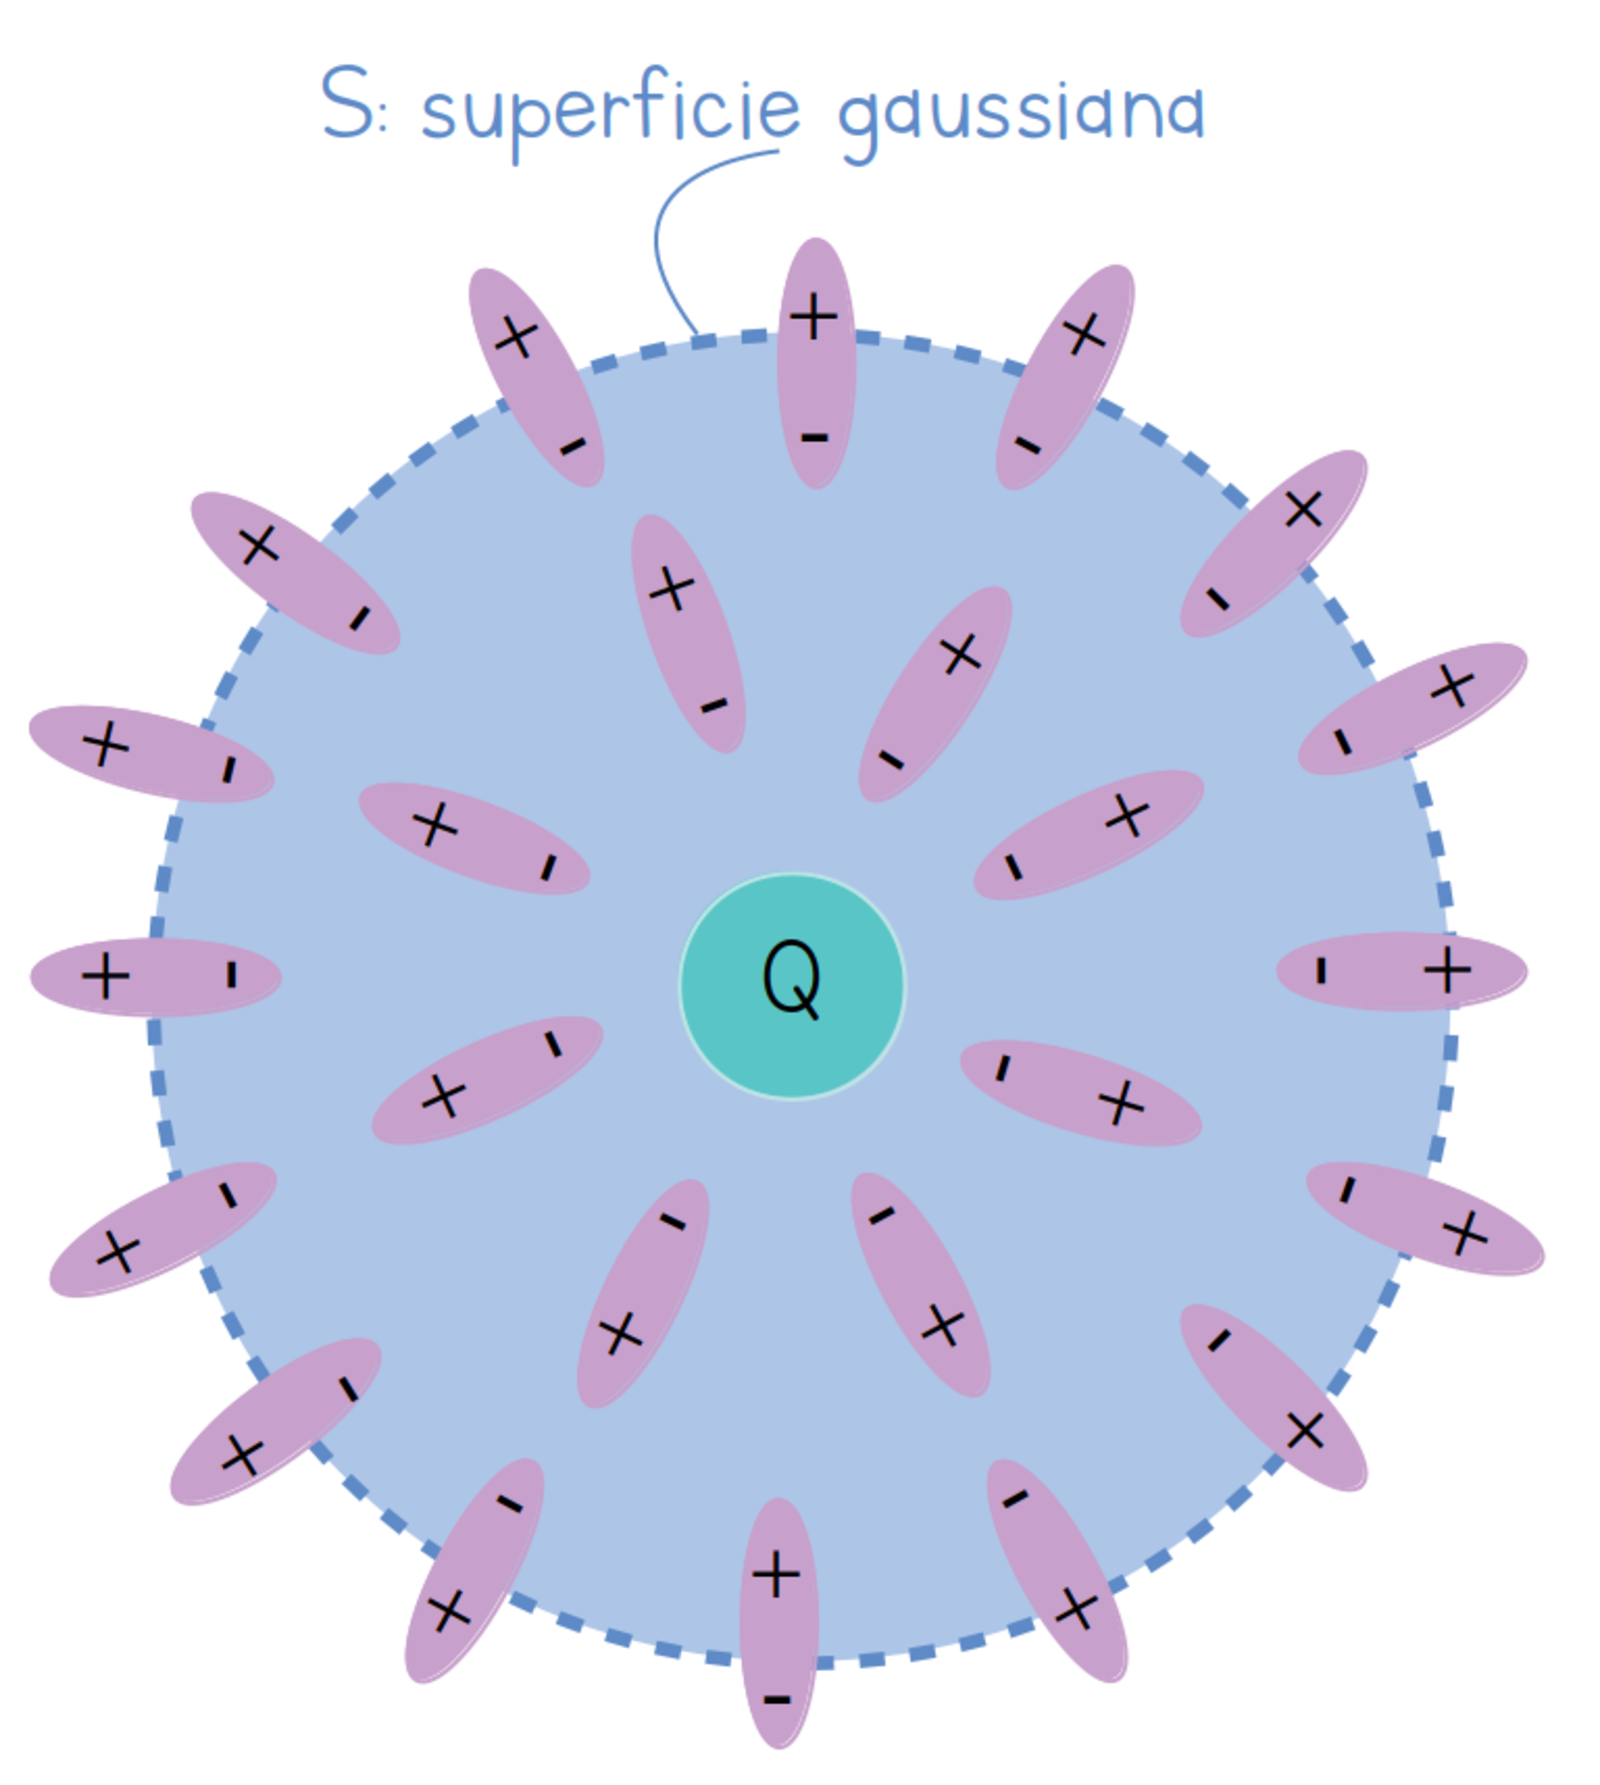
\includegraphics[width=7cm]{figures/fig2}
  \caption{Carga puntual Q en fluido dieléctrico.}
  \label{fig:fig2}
\end{figure}
\sepline

{\color{RedViolet}
  5. a) Considere una frontera entre dos dieléctricos. Utilice la ley de Gauss para encontrar la condición de frontera para $\bar{D}$.
  \\
  b) Utilice el carácter conservativo de $\bar{E}$ y encuentre la condición de frontera para $\bar{E}$.
}
\\
\\
  {\color{WildStrawberry}Solución a):}
  \\
  Dados dos medios diferentes: 1 y 2 (Figura 3), si se supone que existe una densidad de carga externa $\sigma$ que pude variar de un punto a otro que atraviese la interfaz, se pude construir una superficie $S$ con forma de cilindro, cuya altura es despreciable respecto a los diámetros, que tiene un área $\Delta S$ en cada tapa (superior e inferior) y encierra una carga:
  \begin{equation*}
    \sigma \Delta S +\frac{1}{2}(\rho_{1}+\rho_{2})*volumen=Q
  \end{equation*}
  suponiendo que el cilindro está centrado en la interfaz. Si se considera que el volumen es muy pequeño:
  \begin{equation}
    \sigma \Delta S=Q
  \end{equation}

 \begin{figure}[h!]
  \centering
    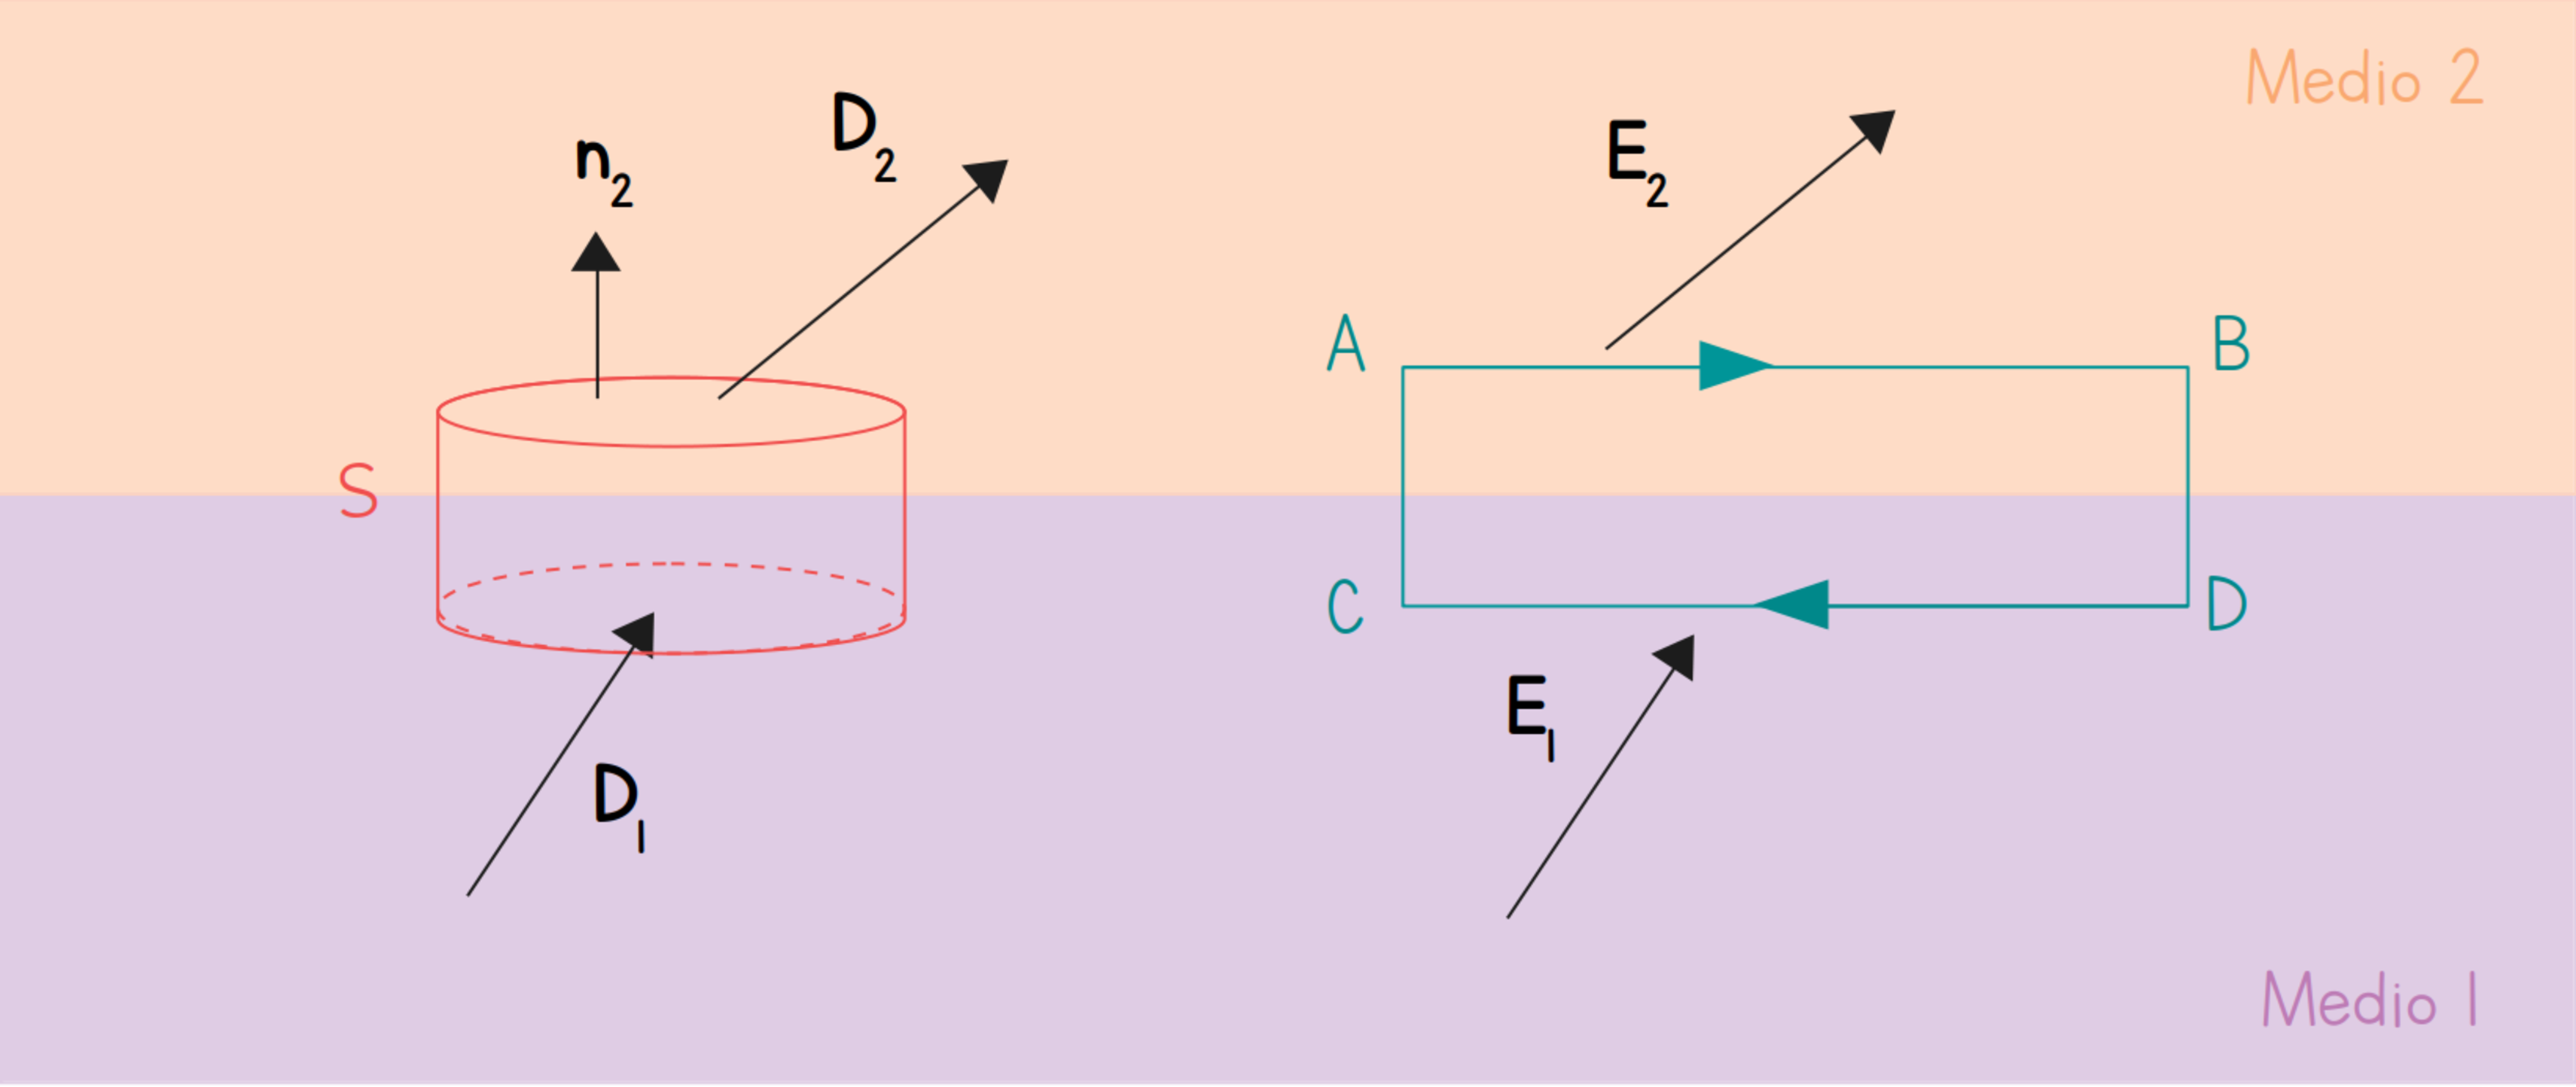
\includegraphics[width=10cm]{figures/2medios}
  \caption{Campos $\bar{E}$ y $\bar{D}$ en dos medios dieléctricos.}
  \label{fig:fig3}
\end{figure}

  
  Usando la Ley de Gauss, (9), en la superficie $S$ se tiene:
  \begin{equation*}
    \oint_{S}\bar{D}\cdot \hat{n}\,da=\int_{Tapa\,sup.}\bar{D}\cdot \hat{n}\,da+\int_{Tapa\,inf.}\bar{D}\cdot \hat{n}\,da+\int_{Lat.}\bar{D}\cdot \hat{n}\,da=Q
  \end{equation*}
  dado que la altura del cilindro tiene a $0$ la  integral correspondiente al lateral se va a $0$, además si el diámetro es lo suficientemente pequeño, los vectores $\bar{D}_{2}$ y $\bar{D}_{1}$ no cambian en la superficie, y pueden salir de las integrales:
  
  \begin{equation*} 
  \rightarrow \,\,\, \int_{Tapa\,sup.}\bar{D}_{2}\cdot \hat{n}_{2}\,da+\int_{Tapa\,inf.}\bar{D}_{1}\cdot \hat{n}_{1}\,da=\bar{D}_{2}\cdot \hat{n}_{2}\int_{Tapa\,sup.}\,da+\bar{D}_{1}\cdot \hat{n}_{1}\,da\int_{Tapa\,inf.}=Q
  \end{equation*}

   \begin{equation*} 
  \rightarrow \,\,\, \bar{D}_{2}\cdot \hat{n}_{2}\Delta S + \bar{D}_{1}\cdot \hat{n}_{1}\Delta S=Q
   \end{equation*}
   
   además $\hat{n}_{1}\,=\,-\hat{n}_{2}$, (el vector normal a la tapa inferior es el negativo de el vector normal a la tapa superior); y sustituyendo $Q$ con (25), se obtiene:

   \begin{equation}
	\tcboxmath[colback=Salmon!25!white,colframe=Salmon, title=\centering Condición de frontera para $\bar{D}$]
	{ (\bar{D}_{2}-\bar{D}_{1})\cdot \hat{n}_{2}=\sigma}
   \end{equation}
La ecuación (26) es la condición de frontera entre dos dieléctricos.y
   \\
   \\
   
  {\color{WildStrawberry}Solución b):}
  \\
  Debido a que $\bar{E}$ es conservativo:
  \begin{equation}
    \oint_{\alpha} \bar{E} \cdot d\bar{l}=0
  \end{equation}
  Usando este resultado para la trayectoria $ABCD$ en la Figura 3 se tiene:

  \begin{equation*}
    \oint_{\alpha}\bar{E} \cdot d\bar{l}=\int_{A\rightarrow B}\bar{E} \cdot d\bar{l}+\int_{B\rightarrow D}\bar{E} \cdot d\bar{l}+\int_{D\rightarrow C}\bar{E} \cdot d\bar{l}+\int_{C\rightarrow A}\bar{E} \cdot d\bar{l}=0
    \end{equation*}
  suponiendo que las longitudes $BD$ y $CA$ son despreciables, y que las longitudes de $AB$ y $DC$ son $\Delta l$ en donde los vectores $\bar{E}_{2}$ y $\bar{E}_{1}$ no cambian, se tiene:
  \begin{equation*}
    \int_{A\rightarrow B}\bar{E}_{2} \cdot d\bar{l}+\int_{D\rightarrow C}\bar{E}_{1} \cdot d\bar{l}=0
  \end{equation*}
   \begin{equation*}
    \rightarrow\,\,\,\bar{E}_{2} (\bar{\Delta l})+\bar{E}_{1}(-\bar{\Delta l})=0
   \end{equation*}
   así:
   \begin{equation}
	\tcboxmath[colback=Salmon!25!white,colframe=Salmon, title=\centering Condición de frontera para $\bar{E}$]
	{ (\bar{E}_{2}-\bar{E}_{1})\cdot \bar{\Delta l}=0}
   \end{equation}
   La ecuación (28) es la condición de frontera para el campo $\bar{E}$, y significa que la componente tangencial del campo eléctrico es continua al atravesar una zona interfacial entre dos dieléctricos.
   \\

\sepline
{\color{RedViolet}
  6. Con el Teorema de la Divergencia demuestre:
  \begin{equation}
    \bar{\nabla} \cdot \bar{D}(\bar{r})=\rho_{libre}(\bar{r})\,\,\,\,y\,\,\,\, \nabla^{2}V(\bar{r})=-\frac{\rho_{libre}(\bar{r})}{\epsilon}
  \end{equation}
  donde el potencial es:
  \begin{equation}
    V(\bar{r})=-\int \bar{E}(\bar{r})\cdot d\bar{l}
  \end{equation}
  }
\\
\\
  {\color{WildStrawberry}Solución:}
  \\
  De la ecuación (9) se tiene:
  \begin{equation*}
    \oint_S \bar{D} \cdot d\bar{a}=Q_{libre}
  \end{equation*}
  además:
  \begin{equation*}
    Q_{libre}=\int_{V}\rho_{libre}\,dv
  \end{equation*}
  aplicando el Teorema de la Divergencia:
 \begin{equation*}
    \oint_S \bar{D} \cdot d\bar{a}=\int_{V}(\bar{\nabla}\cdot\bar{D})\,dv=Q
  \end{equation*}   
  \begin{equation*}
    \rightarrow\,\,\,\int_{V}(\bar{\nabla}\cdot\bar{D})\,dv=\int_{V}\rho_{libre}\,dv\,\,\,\rightarrow\,\,\, \int_{V} (\bar{\nabla}\cdot\bar{D}-\rho_{libre})\,dv=0
  \end{equation*}
  dado que la última igualdad se da para todo volumen $V$, se tiene:

   \begin{equation}
	\tcboxmath[colback=Salmon!25!white,colframe=Salmon, title=\centering Ley de Gauss para dieléctricos:]
	{ \bar{\nabla} \cdot \bar{D}(\bar{r})=\rho_{libre}(\bar{r}) }
   \end{equation}
   Por otro lado, sustituyendo $\bar{D}$ de (20) en (31) se obtiene:
   \begin{equation*}
     \bar{\nabla}\cdot \epsilon \bar{E}=\rho_{libre}\,\,\,\rightarrow\,\,\, \bar{\nabla}\cdot \bar{E}=\frac{\rho_{libre}}{\epsilon}
   \end{equation*}


   además, por (30):
    \begin{equation*}
     \bar{E}=-\nabla V
    \end{equation*}
    sustituyendo esto en (32) se tiene:
    \begin{equation*}
      \bar{\nabla}\cdot (-\nabla V)=\frac{\rho_{libre}}{\epsilon}
    \end{equation*}
    así, finalmente se llega a:

     \begin{equation}
	\tcboxmath[colback=Salmon!25!white,colframe=Salmon, title=\centering Ecuación de Poisson:]
	{\nabla^{2}V(\bar{r})=-\frac{\rho_{libre}(\bar{r})}{\epsilon}}
      \end{equation}

      
\begin{thebibliography}{99}
\bibitem{Reitz}J. Reitz, \textit{Fundations of Electromagnetic Theory}, ADDISON-WESLEY, United States of America.
\end{thebibliography}


\end{document} 
